\newpage
\chapter{Nombres Complexes}
\vspace{3mm} %5mm vertical space
\section{Conversion polaire - cartésienne}
\vspace{3mm} %5mm vertical space

\textbf{Définition du module} \\

le module noté $|Z|$ est la longueur du segment (rayon). Elle peut être mesurée  grâce à la formule de pythagore ($\sqrt{a²+b²}$). \\


\vspace{5mm} %5mm vertical space
\textbf{Représentation Géographique} \\

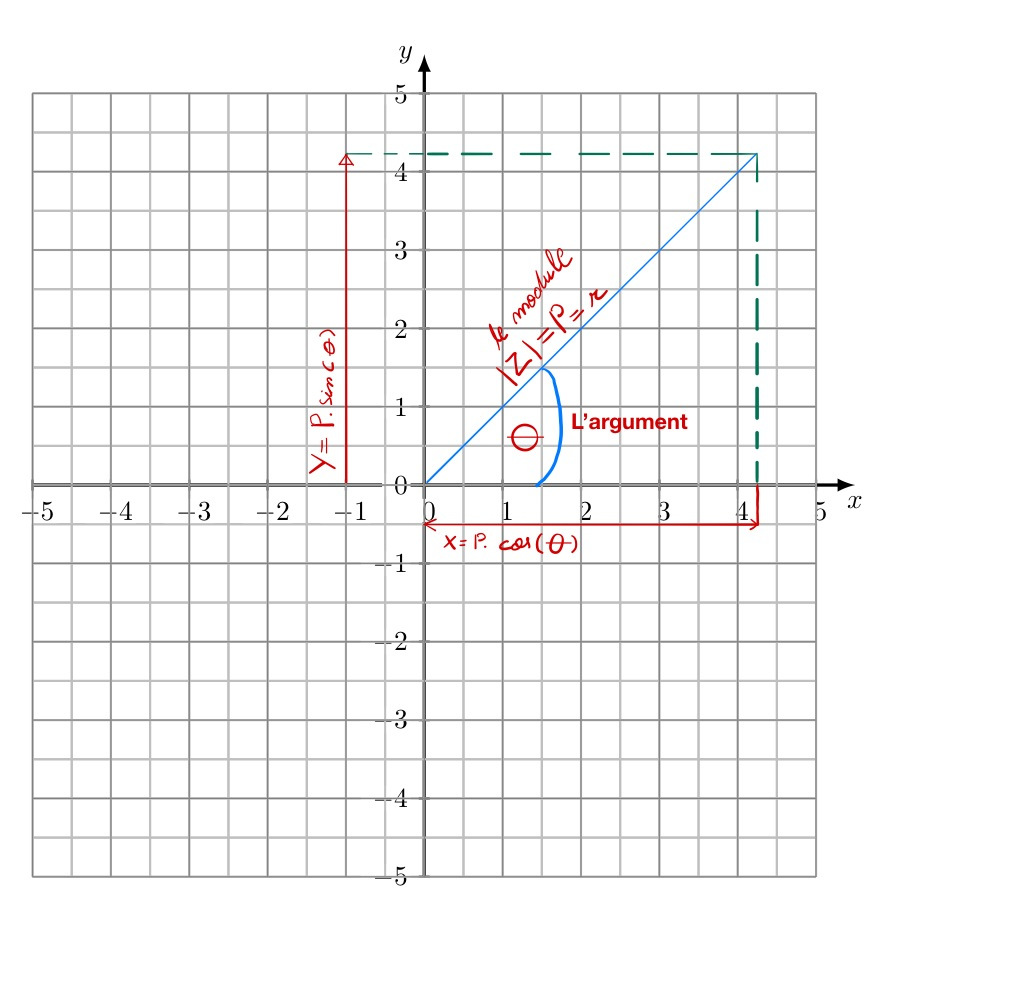
\includegraphics[scale=1.5]{cart-mod}

\textbf{Démonstration}\\

$|Z| = \rho cos(\theta)+ \rho sin(\theta) *i$ \\
$|Z| = \sqrt(\rho^{2} cos(\theta)^{2}+ \rho^{2} sin(\theta)^{2})$ \\
$|Z| = \sqrt(\rho^{2} cos(\theta)^{2}+ sin(\theta))*i $ \\
$|Z| = \sqrt(\rho^{2}) $ \\
$|Z| = \rho $ \\

$\rho$ est le module et $\theta$ est l'argument \\
$Z = P(cos(\theta) + sin(\theta)*i )$ ou $Z= P(cis(\theta))$\\

\newpage

\section{Conversion Cartésienne - Polaire}
\vspace{3mm} %5mm vertical space

$\rho$ = $\sqrt{x²+y²}$ \\

\textbf{Démonstration Géométriquement} \\

Nous pouvons voir que $\theta$ est modifié en fonction de X et de Y que si nous dessinons un cercle, nous pouvons voir que le segment Y est une tangeante au cercle de rayon X. \\

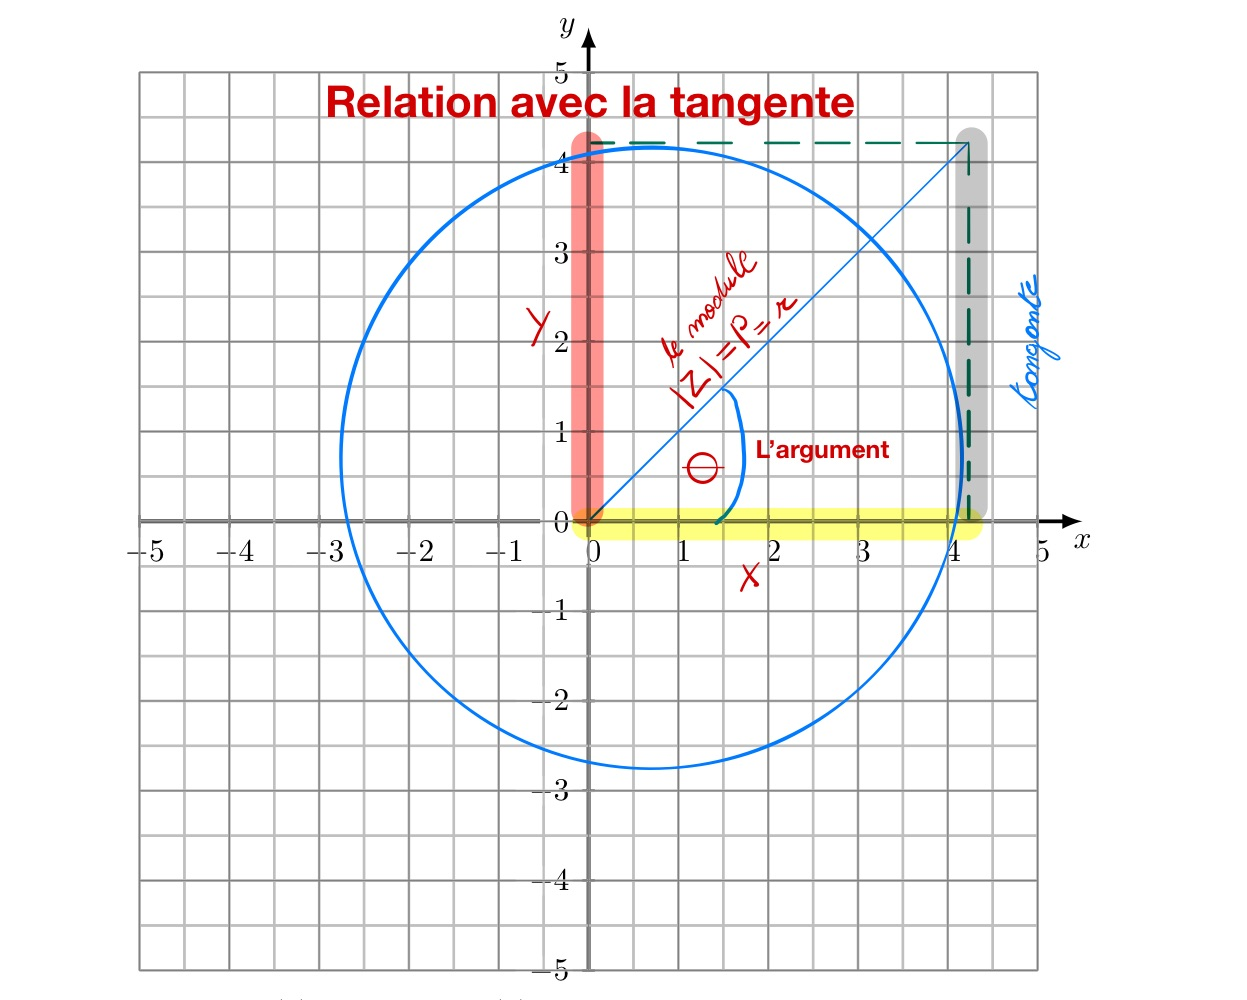
\includegraphics[scale=0.3]{cart-tg}

$X=\rho * cos(\theta)$ $ $ $ Y=\rho * sin(\theta)$

\vspace{5mm} %5mm vertical space
\textbf{Démonstration Algébriquement} \\

$\frac{Y}{X}$ = $\frac{\rho * sin(\theta)}{\rho * cos(\theta)}$ \\
$\frac{Y}{X}$ = $\frac{sin(\theta)}{cos(\theta)}$ \\
$\frac{Y}{X}$ = tg($\theta)$ \\

\vspace{5mm} %5mm vertical space
\textbf{Conclusion} \\

$\theta = arctg(\frac{Y}{X})$ \\
$tg(\theta) = \frac{Y}{X}$ \\


\newpage

\section{Conversion cartésienne/polaire - exponentielle}
\vspace{3mm} %5mm vertical space

tout nombre complexes peut s'écrire sous la formes : $\rho * e^{i\theta}$ \\

\textbf{Ecriture cartésienne} \\

$1+\sqrt{3}i$ = x + yi \\

\vspace{5mm}
\textbf{Etape 1: Trouver $\rho$ (calcul du module)} \\

$\rho = \sqrt{x^{2} + y^{2}}$ \\

$\rho = \sqrt{1^{2} + \sqrt{3}^{2}}$ \\

$\rho = \sqrt{1 + 3}$ \\

$\rho = \sqrt{4 => 2^{2}}$ \\

$\rho = 2$ \\

\vspace{5mm}
\textbf{Etape 2: Trouver $\theta$ (calcul de l'argument)} \\

$\theta = artg(\frac{y}{x})$ \\

$\theta = arctg(\frac{1}{\sqrt{3}})$ \\

$tg(\theta) = \frac{1}{\sqrt{3}} * \frac{\sqrt{3}}{\sqrt{3}}$ \\

$tg(\theta) = \frac{1\sqrt{3}}{\sqrt{3}^{2}}$ \\

$tg(\theta) = \frac{\sqrt{3}}{3})$ ou $artg(\frac{\pi}{6}) $ \\

$tg(\theta) = \frac{\pi}{6} $ \\


\vspace{5mm}
\textbf{Etape 3: Ecriture sous le format exponentielle} \\

$2e^{\frac{\pi}{6}i}$


\newpage
\section{Conversion exponentielle - polaire/cartésienne }
\vspace{3mm} %5mm vertical space

\textbf{Ecriture exponentielle} \\

$e^{1+\frac{\pi}{2}i}$ \\

\textbf{Simplification} \\

$e^{1+\frac{\pi}{2}i}$ \\

$e^{1} + e^{\frac{\pi}{2}i}$ \\

$e*cis(\frac{\pi}{2})$ \\

$e*(cos(\frac{\pi}{2}) + i*sin(\frac{\pi}{2})) $ \\

$e*(cos(\frac{\pi}{2}) + i*sin(\frac{\pi}{2})) $ \\

$e*(0 + i*1) $ \\

$e*i $ \\


\newpage
\section{Nombre Complexes addition}
\vspace{3mm} %5mm vertical space

$(4 * cis(45^{\circ} )) + (5 * cis(\frac{\pi}{3}))$

\vspace{10mm}
\textbf{Calcul du module}
\vspace{5mm}

$\rho = \sqrt{\rho_{1}^{2} + \rho_{2}^{2} + \rho_{1} \rho_{2} cos(\theta_{1} - \theta_{2}) }$ \\

$\rho = \sqrt{4^{2} + 5^{2} + 2 * 4 * 5 cos(45^{\circ} - 60^{\circ})}$ \\

$\rho = \sqrt{41 + 40 * 0,96592582628}$ \\

$\rho = \sqrt{79,6370330512}$ \\

$\rho = 8,923958373457376 $ \\

\vspace{6mm}
\textbf{Calcul de l'argument}
\vspace{5mm}

$\theta = arctg(\frac{\rho_{1}sin(\theta_{1}) + \rho_{2}sin(\theta_{2})} {\rho_{1}cos(\theta_{1}) + \rho_{2}cos(\theta_{2})} )$ \\

$\theta = arctg(\frac{4sin(45^{\circ}) + 5sin(60^{\circ})} {4cos(45^{\circ}) + 5cos(60^{\circ})} )$ \\

$\theta = arctg(\frac{4\frac{\sqrt{2}}{2}) + 5\frac{\sqrt{3}}{2} } {4\frac{\sqrt{2}}{2}) + 5\frac{1}{2}})$ \\

$\theta = arctg(1.3434647741399612)$ \\

$\theta = arctg(53.3380661^{\circ})$ \\

\vspace{6mm}
\textbf{Solution}
\vspace{5mm}

$|Z| = 8,923 cis(53.338^{\circ})$


\newpage
\section{Nombre Complexes soustraction}
\vspace{3mm} %5mm vertical space

$(4 * cis(45^{\circ} )) - (5 * cis(\frac{\pi}{3}))$


\vspace{6mm}
\textbf{Calcul du modules}
\vspace{5mm}

$\rho = \sqrt{\rho_{1}^{2} + \rho_{2}^{2} + 2*\rho_{1}*\rho_{2} cos(\theta_{1} -  \theta_{2})}$ \\

$\rho = \sqrt{4^{2} + 5^{2} +2*4*5* cos(45^{\circ} - \frac{\pi}{3})}$ \\

$\rho = \sqrt{4^{2} + 5^{2} + 40* cos(45^{\circ} - 60^{\circ})}$ \\

$\rho = \sqrt{16 + 25 + 40* 0,965925826}$ \\

$\rho = \sqrt{79,637033052}$ \\

$\rho = 8,923958374$ \\

\vspace{4mm}
\textbf{Calcul de l'argument}
\vspace{5mm}

$\theta = arctg(\frac{\rho_{1}*sin(\theta_{1}) - \rho_{2}*sin(\theta_{2})}{\rho_{1}*cos(\theta_{1}) - \rho_{2}*cos(\theta_{2})})$ \\

$\theta = arctg(\frac{4*sin(45^{\circ}) - 5*sin(\frac{\pi}{3})}{4*cos(45^{\circ}) - 5*cos(\frac{\pi}{3})})$ \\

$tg(\theta) = \frac{4*sin(45^{\circ}) - 5*sin(60^{\circ})}{4*cos(45^{\circ}) - 5*cos(60^{\circ})}$ \\

$tg(\theta) = \frac{4\frac{\sqrt{2}}{2} - 5\frac{\sqrt{3}}{2} } {4*\frac{1}{2} - 5 * \frac{\sqrt{2}}{2}}$ \\

$tg(\theta) = \frac{2\sqrt{2} - \frac{5\sqrt{3}}{2} } {2 - \frac{5\sqrt{2}}{2} }$ \\

$tg(\theta) = \frac{\frac{4\sqrt{2} - 5\sqrt{3}}{2}} {\frac{4 - 5\sqrt{3}}{2} }$ \\

$tg(\theta) = \frac{4\sqrt{2} - 5\sqrt{3}} {4 - 5\sqrt{3} }$ \\

$tg(\theta) = - \frac{(4\sqrt{2} - 5\sqrt{3}) * (4\sqrt{2} - 5\sqrt{3})}{59}$ \\

$tg(\theta) = - \frac{(16\sqrt{2} + 20\sqrt{6} - 20\sqrt{3} - 75)} {59}$ \\

$tg(\theta) = 0,644471$ \\

$tg(\theta) = 36,93^{\circ}$ \\


\vspace{6mm}
\textbf{Solution}
\vspace{5mm}

$|Z| = 8,923958374*cis(36,93^{\circ})$ \\

\newpage
\section{Nombre Complexes multiplication}
\vspace{3mm} %5mm vertical space

$(4 * cis(45^{\circ} )) * (5 * cis(\frac{\pi}{3}))$ \\

$|Z| = \rho_{1}\rho_{2}( cos(\theta_{1} + \theta_{2}) + i*(sin(\theta_{1} + \theta_{2})) )$ \\

$|Z| = (\rho_{1}\rho_{2})*cis(\theta_{1} + \theta_{2})$ \\


\vspace{6mm}
\textbf{Calcul du modules}
\vspace{5mm}

$\rho = \rho_{1}\rho_{2}$ \\

$\rho = 4*5 $ \\

$\rho = 20 $ \\

\vspace{6mm}
\textbf{Calcul de l'argument}
\vspace{5mm}

$\theta = \theta_{1}+\theta_{2}$ \\

$\theta = 45^{\circ} + \frac{\pi}{3}$ \\

$\theta = 45^{\circ} + 60^{\circ}$ \\

$\theta = 105^{\circ}$ \\

\vspace{6mm}
\textbf{Solution}
\vspace{5mm}

$|Z| = 20 * cis(105^{\circ})$

\newpage
\section{Nombre Complexes division}
\vspace{3mm} %5mm vertical space

$\frac{(4 * cis(45^{\circ} ))} {(5 * cis(\frac{\pi}{3}))} $ \\

$|Z| = (\frac{\rho_{1}}{\rho_{2}})* cis(\theta_{1} - \theta_{2})$ \\

\vspace{6mm}
\textbf{Calcul du modules}
\vspace{5mm}

$\rho = \frac{4}{5}$ \\

\vspace{6mm}
\textbf{Calcul de l'argument}
\vspace{5mm}

$\theta = 45^{\circ} - \frac{\pi}{3} $ \\

$\theta = 45^{\circ} - 60^{\circ} $ \\

$\theta = - 15^{\circ} $ \\

\vspace{6mm}
\textbf{Solution}
\vspace{5mm}

$ |Z| = \frac{4}{5} * cis(- 15^{\circ})$ \\
